\subsection{Non-uniformities in HWP optical properties}

\paragraph{Description:}
Non-uniformities (e.g.: small patches of the HWP surface with lower or higher transmission/reflection/absorption with respect to the overall surface) in the optical properties of the HWP produce discontinuities in the output signal. The size of this effect is dependent on where the HWP is located in the optics. If the all detectors see the full HWP, this effect is minimized, but if detectors see different parts of the HWP, then this effect is more significant.

\textbf{What types of systematic effects does this lead to? Leakage? Gain variation?}



\paragraph{Plan to model and/or measure:}
Different approaches can be used to estimate/measure this systematic from its many sources, including EM calculation with gap (or dust) between layers or thickness error, 3D shape measurements for various points on the HWP, and measurements of the
HWP synchronous signal across the array. The HWP can be additionally characterized with FTS and reflectometry measurements. The importance of non-uniformities is minimized when the detector beams are equivalent in size to the HWP at the HWP.

\textbf{Do we need to include some sort of beam modeling here?}

This effect is expected to be relatively small, but we should model it to check, making the SRF a 3.

\paragraph{Uncertainty/Range:}
\textbf{Based on the location of the HWP in the SAC, how significant do we expect this effect to be?}

\begin{figure}
\begin{center}
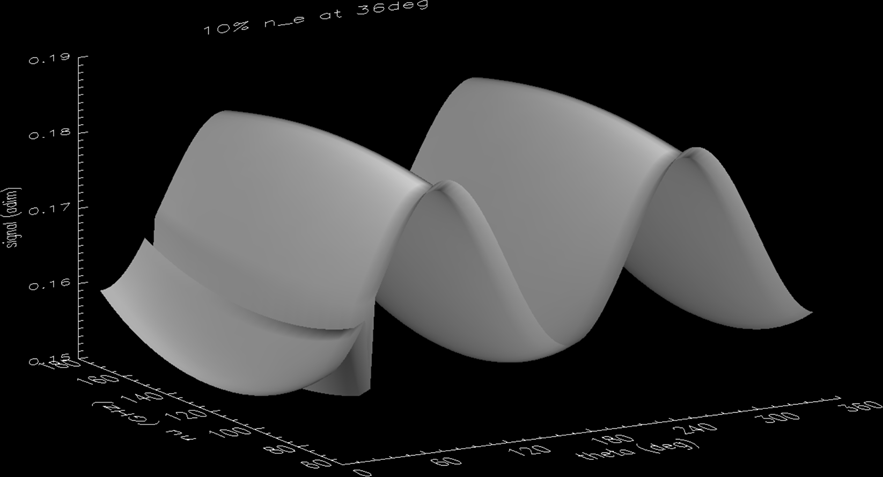
\includegraphics[width=0.6\linewidth]{hwp_nonuniform.png}
\caption{2$f$ signal from a (1,0,0,0) Stokes vector incident on a HWP with a localized non-uniformity: a discontinuous increase of
10$\%$ of the extraordinary index at theta=36${\circ}$.}\label{hwpnonuniform}
\end{center}
\end{figure}

\paragraph{Parameterization:}
The simplest way to parameterize this is to introduce a discontinuous variation in one HWP optical property. In a test model we have introduced a 10$\%$ increase of the extraordinary index when the HWP
is rotating at 36deg (Fig.\,\ref{hwpnonuniform}). 


\textbf{How to discontinuities in the optical properties filter impact the science? How do we parameterize that?}
